\documentclass{beamer}

\usepackage{xcolor}
\usepackage{graphicx}
\usepackage{varwidth}
% \usepackage{caption}

\usepackage{subcaption}
\usepackage{media9}
\usepackage{multimedia}

\usepackage{amsfonts,amsmath,amssymb}
\usepackage{blkarray,booktabs,bigstrut}

\usepackage{pgfplots}
\usepackage{tikz}
\usepackage{filecontents}
\usepackage{lmodern}

\usetikzlibrary{hobby}
\usetikzlibrary{decorations.shapes}
\usetikzlibrary{shadows.blur}

\definecolor{NvidiaGreen}{RGB}{118, 185, 0}

\usetheme{Madrid}
\setbeamertemplate{navigation symbols}{}

% Set the colors for various Beamer elements
\setbeamercolor{title}{fg=black, bg=NvidiaGreen} 
\setbeamercolor{frametitle}{fg=black, bg=NvidiaGreen} 
\setbeamercolor{item}{fg=black, bg=NvidiaGreen} 
\setbeamercolor{section in toc}{fg=black, bg=NvidiaGreen}
\setbeamercolor{author}{fg=white, 
        % bg=NvidiaGreen
    }
\setbeamercolor{date}{fg=white, 
        % bg=NvidiaGreen
    }

% Set the background to white for a clean presentation
\setbeamercolor{background canvas}{bg=white}

% #########################################################################################
% #########################################################################################
% Title
% #########################################################################################
% #########################################################################################

\begin{document}
{
\setbeamertemplate{background} 
{
    \includegraphics[width=\paperwidth,height=\paperheight]{images/Screenshot_9-12-2024_212019_.jpeg}
}
\title{\textbf{Lecture 15 - Spectral Clustering}}
\author[]{\textbf{Renan Monteiro Barbosa}}
% \date{\today}
\date[]{\textbf{2025}}
\maketitle
}

% #########################################################################################
% #########################################################################################
% Slide 1 - Intro
% #########################################################################################
% #########################################################################################

\section{Spectral Clustering}
\begin{frame}
\frametitle{\textbf{Spectral Clustering} }

Let G be a graph, $G(V,E)$, where $V = \left\{1,2,3, \cdots, n\right\}$ \vspace{0.2 cm}

The Laplacian matrix: 
% \parbox{4em}
\[
L_{G} = \underbrace{D_{G}}_{\parbox{3cm}{\centering Diagonal matrix \\[-3pt] with degrees of each vertex}} - \underbrace{A_{G}}_{\text{adjancency matrix}}
\]

$L_{G}$ is a PSD Matrix whose eigenvalues are

\begin{equation*}
    0 = \lambda_1 \leq \underbrace{\lambda_2}_{\text{Fiedler value}}\leq \lambda_3 \leq \cdots \leq \lambda_n
\end{equation*}

An eigenvector with eigenvalue $\lambda_2$ is called the \underline{Fiedler vector} of $\vec{W}$.


\end{frame}

% #########################################################################################
% #########################################################################################
% Slide 2 - Intro
% #########################################################################################
% #########################################################################################

\section{Spectral Clustering}
\begin{frame}
\frametitle{\textbf{Spectral Clustering} }

We will use $\vec{W}$, $L_{G}$ to understand clusters in a graph. \vspace{0.5 cm}

% Need to draw the graph clusters and draw the circle

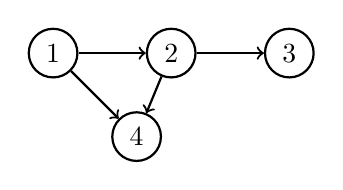
\begin{tikzpicture}[node distance={15mm}, thick, main/.style = {draw, circle}] 
    \node[main] (1) {$1$}; 
    \node[main] (2) [right of=1] {$2$}; 
    \node[main] (3) [right of=2] {$3$}; 
    \node[main] (4) [below right of=1] {$4$}; 
    \draw[->] (1) -- (2); 
    \draw[->] (1) -- (4);  
    \draw[->] (2) -- (3); 
    \draw[->] (2) -- (4); 
\end{tikzpicture}

$A = \left\{4,5,6,7,8\right\} , |A| = 5$

Notation

If X, Y are sets $X \ Y = \left\{x \in X | x \notin Y\right\}$

$|x| = \text{size of x}$



\end{frame}

% #########################################################################################
% #########################################################################################
% Slide 3 - Cut
% #########################################################################################
% #########################################################################################

\section{Cut}
\begin{frame}
\frametitle{\textbf{Cut} }
\textbf{Definition} \vspace{0.2 cm}

A cut is G is a partition of V into two sets, A and V \ A, when $A V$. (The cut induced by A)

\textbf{Notation} \vspace{0.2 cm}

If $X,Y V$, let E(X,Y) denote all edges with one certex in X and one vertex in Y.

$E(A, V \ A) = \left\{ \left\{1,6\right\} \right\}$


Definition

The density of the cut induced by A is:



\end{frame}

% #########################################################################################
% #########################################################################################
% Slide 4 - Sparsest cut
% #########################################################################################
% #########################################################################################

\section{Sparsest cut}
\begin{frame}
\frametitle{\textbf{Sparsest cut} }
Definition: \vspace{0.2 cm}

Let denote the smallest possible desnity of ca cut in G. Any cut with density is called a sparesest cut in G.

\end{frame}

% #########################################################################################
% #########################################################################################
% Slide 5 - Define BG
% #########################################################################################
% #########################################################################################

\section{Define BG}
\begin{frame}
\frametitle{\textbf{Define BG} }

Define the matrix $B_{G}$, the \underline{"directed" node-edge incidence matrix of G}.

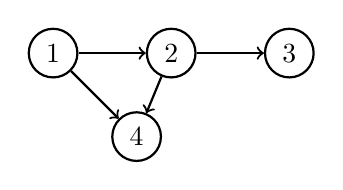
\begin{tikzpicture}[node distance={15mm}, thick, main/.style = {draw, circle}] 
    \node[main] (1) {$1$}; 
    \node[main] (2) [right of=1] {$2$}; 
    \node[main] (3) [right of=2] {$3$}; 
    \node[main] (4) [below right of=1] {$4$}; 
    \draw[->] (1) -- (2); 
    \draw[->] (1) -- (4);  
    \draw[->] (2) -- (3); 
    \draw[->] (2) -- (4); 
\end{tikzpicture}

pick a direction for each edge

% TODO - figure out how to draw Arrows connecting stuff.

rows indexed by nodes

columns indexed by edges of G

\[
    B_{G} = 
    \begin{blockarray}{ccccc}
        & 12  & 14 & 23 & 24 \\
    \begin{block}{c[cccc]}
    1   & 1  & 1  & 0  & 0  \\
    2   & -1 & 0  & 1  & 1  \\
    3   & 0  & 0  & -1 & 0  \\
    4   & 0  & -1 & 0  & -1 \\
    \end{block}
    \end{blockarray}\vspace*{-1.25\baselineskip}
\]

In the column indexed by the directed edge ij, we put 1 in row i and -1 in row j.

$L_{G} = B^{T}B$

\end{frame}

% #########################################################################################
% #########################################################################################
% Slide 6 - Define BG
% #########################################################################################
% #########################################################################################

\section{Define BG}
\begin{frame}
\frametitle{\textbf{Define BG} }

$L_{G} = B_{G} \cdot B_{G}^{T}$

% TODO - Add notes on the bottom of each Matrix

\begin{equation*}
    \left\lbrack\begin{array}{cccc}
        1  & 1  & 0  & 0  \\
        -1 & 0  & 1  & 1  \\
        0  & 0  & -1 & 0  \\
        0  & -1 & 0  & -1 \\
    \end{array}\right\rbrack
    \cdot
    \left\lbrack\begin{array}{cccc}
        1 & -1 & 0  & 0  \\
        1 &  0 & 0  & -1  \\
        0 &  1 & -1 & 0  \\
        0 &  1 & 0  & -1 \\
    \end{array}\right\rbrack
    =
    \left\lbrack\begin{array}{cccc}
        2  & -1 & 0  & -1 \\
        -1 &  3 & -1 & -1 \\
        0  & -1 & 1  & 0  \\
        -1 & -1 & 0  & 2  \\
    \end{array}\right\rbrack
\end{equation*}

If you get $i^{th}$ row and $i^{th}$ column, $1^2$ or $(-1)^2$ for every edge incident to i. So the sum $d_{i}$.

$i^{th}$ row and $j^{th}$ column (if $i \neq j$ ) if ij is on edge, you will get $1(-1) = -1$

Therefore, $L_{G}$ is PSD.

% \[
%     B_{G} \cdot B_{G}^{T} = 
%     \begin{blockarray}{ccccc}
%         & 12  & 14 & 23 & 24 \\
%     \begin{block}{c[cccc]}
%     1   & 1  & 1  & 0  & 0  \\
%     2   & -1 & 0  & 1  & 1  \\
%     3   & 0  & 0  & -1 & 0  \\
%     4   & 0  & -1 & 0  & -1 \\
%     \end{block}
%     \end{blockarray}\vspace*{-1.25\baselineskip}
% \]


\end{frame}

% #########################################################################################
% #########################################################################################
% Slide 7 - Lemma
% #########################################################################################
% #########################################################################################

\section{Lemma}
\begin{frame}
\frametitle{\textbf{Lemma} }
Lemma: \vspace{0.2 cm}

If G is a graph, the Laplacian $L_{G}$ is PSD and its eigenvalues are:

\begin{equation*}
    0 = \lambda_{1} \leq \lambda_{2} \leq \lambda_{3} \leq \cdots \leq \lambda_{n}
\end{equation*}

and $\vec{1}$ is an eigenvector of $L_{G}$ with eigenvalue 0.

Since $L_{G}$ is PSD, the $\vec{x}^{T}L_{G}\vec{x} \geq 0$, $\forall \vec{x} \in \mathbb{R}^n$

\end{frame}

% #########################################################################################
% #########################################################################################
% Slide 8 - Lemma
% #########################################################################################
% #########################################################################################

\section{Lemma}
\begin{frame}
\frametitle{\textbf{Lemma} }
PwP: \vspace{0.2 cm}

Let $G=\left([n], E\right)$ be the graph with vertices [n] and edge set E. If $\vec{x}=\left(x_1, \cdots , x_n\right)^T$. \vspace{0.2 cm}

\begin{equation*}
    \vec{x}^{T}L_{G}\vec{x} = \sum_{\left\{i,j\right\} \in E}\left(x_{i}-x_{j}\right)^2
\end{equation*}

Proof \vspace{0.2 cm}

We know that $L_{G}=B_{G}B_{G}^{T}$. So $\vec{x}^{T}L_{G}\vec{x} = \vec{x}^{T}B_{G}B_{G}^{T}\vec{x}$. \vspace{0.2 cm}

Lets understand $\vec{x}^{T}B_{G}$.\vspace{0.2 cm}

% TODO - Add the vector dot product

So the entries of $\vec{x}^{T}B_{G}$ are all $x_{i}-x{j}$ when ij is an edge of G.

\end{frame}

% #########################################################################################
% #########################################################################################
% Slide 9 - Lemma
% #########################################################################################
% #########################################################################################

\section{Lemma}
\begin{frame}
\frametitle{\textbf{Lemma} }
PwP: \vspace{0.2 cm}

So $\vec{x}^{T}L_{G}\vec{x} = \left(\vec{x}^{T}B_{G}\right) \cdot \left(B_{G}^{T}\vec{x}\right) = \sum_{\left\{i,j\right\} \in E}\left(x_{i}-x_{j}\right)^2$. \vspace{0.2 cm}

Do this for the example:

\end{frame}

% #########################################################################################
% #########################################################################################
% Slide 10 - Connectivity
% #########################################################################################
% #########################################################################################

\section{Connectivity}
\begin{frame}
\frametitle{\textbf{Connectivity} }
Definition: \vspace{0.2 cm}

A Graph is conencted if there is a way to walk from any vertex to any other vertex along the edges of G.

%  TODO - Draw a non-connected Graph

Theorem:

G is connected if and only if $\lambda_2 > 0$.

Proof:

If G is not connected the Graph Laplacian will look like this:

%  TODO - Draw the graph laplacian of a non conencted graph.

\end{frame}

% #########################################################################################
% #########################################################################################
% Slide 11 - Connectivity
% #########################################################################################
% #########################################################################################

\section{Connectivity}
\begin{frame}
\frametitle{\textbf{Connectivity} }
We sort of proved if G is not connected, then $\lambda_2 = 0$. (if G has k components, $\lambda_1 = \lambda_2 = \cdots \lambda_4 = 0$) \vspace{0.2 cm}

We still need t show that if G is connected, $\lambda_2 > 0$.

For a symmetric matrix, $AM(\lambda) = GM(\lambda)$ for an eigenvalues.

So we need to show $GM(0)=1$. Let $\vec{u}$ be an eigenvector with eigenvalue of 0. Then $L_{G}\vec{u}=\vec{0}$.

\begin{equation*}
    0 = \vec{u}^{T}L_{G}\vec{u} = \sum_{\left\{i,j\right\} \in E}\left(u_{i}-u_{j}\right)^2
\end{equation*}

If $u_1 = C$ and {1,k} is an edge, the $u_k = c$. for all edge $ij \in E$.

Similarly if kj is an edge $u_j=c$. Since G is connected $\vec{u} = c \vec{1}$. 

AM, algebraic multiplicity. \vspace{0.2 cm}

GM, geometric multiplicity. \vspace{0.2 cm}

\end{frame}


% #########################################################################################
% #########################################################################################
% Slide XX - Conclusion
% #########################################################################################
% #########################################################################################

\section{Conclusion}
\begin{frame}
\frametitle{Conclusion}

Slight Generalization: \vspace{0.2 cm}

The number of times 0 is on eigenvalue of $L_{G}$ counts the number of conencted components of G.

Fact: \vspace{0.2 cm}

The second eigenvalue $\lambda_2$ is called the spectra gap or the Fiedler value of G.

\end{frame}

% #########################################################################################
% #########################################################################################
% Slide XX - Testing Latex stuff
% #########################################################################################
% #########################################################################################

\section{Testing Latex stuff}
\begin{frame}
\frametitle{\textbf{Testing Latex stuff} }

\[
    \mathbf{\alpha} = 
      \bordermatrix{ & \bar{f_1} & \bar{f_2} & \bar{f_3} \cr
        k_1 & 0 & 0 & 1 \cr
        k_2 & 1 & 0 & 0 \cr
        k_3 & 0 & 0 & 1 \cr
        k_4 & 0 & 1 & 0 } \qquad
\]

\begin{equation*}
    \left\lbrack\begin{array}{cccc}
        2  & -1 & 0  & -1 \\
        -1 & 3  & -1 & -1 \\
        0  & -1 & 1  & 0  \\
        -1 & -1 & 0  & 2  \\
    \end{array}\right\rbrack
\end{equation*}

\end{frame}

% #########################################################################################
% #########################################################################################
% Slide XX - Testing Latex stuff
% #########################################################################################
% #########################################################################################

\section{Testing Latex stuff}
\begin{frame}
\frametitle{\textbf{Testing Latex stuff} }

\[
    \mathbf{\beta} = 
    \begin{blockarray}{cccc}
          & \bar{f_1} & \bar{f_2} & \bar{f_3} \\
        \begin{block}{c(ccc)}
          f_1 & 3 & 2 & 0 \\
          f_2 & 2 & 4 & 2 \\
          f_3 & 5 & 3 & 1 \\
        \end{block}
    \end{blockarray}
\]

\[
    \begin{blockarray}{ccccc}
        & C_1 & C_2 & \dots & C_n \\
    \begin{block}{c[cccc]}
    N_1 & a_{11} & a_{12} & \cdots & a_{1n} \bigstrut[t] \\
    N_2 & a_{21} & a_{22} & \cdots & a_{2n}              \\
        & \vdots & \vdots & \ddots & \vdots              \\
    N_n & a_{n1} & a_{n2} & \cdots & a_{nn} \bigstrut[b] \\
    \end{block}
    \end{blockarray}\vspace*{-1.25\baselineskip}
\]

\[
    \gamma  = 
    \begin{blockarray}{cccccc}
        & \bar{f_1} & \bar{f_2} & \dots & \bar{f_n} \\
    \begin{block}{c[cccc]c}
    k_1 & 0 & 1  & \cdots & 0\bigstrut[t] & =1 \\
    k_2 & 1 & 0  & \cdots & 0 & =1 \\
        & \vdots & \vdots & \ddots & \vdots &\\
    k_n & 0 & 0  & \cdots & 1\bigstrut[b] & =1\\
    \end{block}
        & \leq 4 & \leq 5 & \dots & \leq 10 & \\
    \end{blockarray}\vspace*{-1.25\baselineskip}
\]

\end{frame}

% #########################################################################################
% #########################################################################################
% #########################################################################################
% #########################################################################################

% ⠀⠀⠀⠀⠀⠀⠀⠀⠀⠀⠀⠀⠀⣀⣀⣀⡀⠀⠀⠀⠀⠀⠀⠀⠀⠀
% ⠀⠀⠀⠀⠀⠀⢀⣠⠤⠖⠈⠉⠉⠀⠀⠀⠀⠉⠢⡀⠀⠀⠀⠀⠀⠀
% ⠀⠀⠀⠀⠀⣴⠏⠀⠀⠀⠀⠀⠀⠀⠀⠀⠀⠀⠀⠈⢦⡀⠀⠀⠀⠀
% ⠀⠀⠀⣠⠞⠁⠀⠀⠀⠀⠀⠀⠀⠀⠀⢀⠞⠋⢙⣦⡈⣷⡄⠀⠀⠀
% ⠀⣀⠶⠁⠀⠀⣀⣀⡀⠀⠀⠀⠀⠀⡴⠁⠀⠀⠿⢿⡟⣌⢿⠀⠀⠀
% ⣠⡿⠀⢠⣜⠉⠀⠀⠙⢷⢄⠀⠀⠀⢧⠀⠀⠀⠀⠀⠀⠘⡆⢧⡀⠀
% ⣯⠃⠀⢾⣿⠗⠀⠀⠀⠀⡽⠀⠀⠀⠈⠳⢄⣀⠀⠀⠀⡰⠃⠘⣵⡄
% ⡏⠀⠀⠘⡄⠀⠀⠀⣠⠞⠁⠀⠀⠀⠀⠀⠀⠀⠉⠉⠁⠀⠀⠀⢱⡇
% ⡅⠀⠀⠀⠙⠒⠔⠚⠁⠀⠀⠀⠀⠀⠀⠀⠀⠀⠀⠀⠀⠀⠀⠀⠀⡇
% ⣧⡀⠀⠀⠀⠀⠀⠀⠀⠀⠀⠀⠀⠀⠀⠀⠀⢠⠀⠀⠀⠀⠀⠀⠀⡗
% ⡿⡇⠀⠀⠀⠀⠀⠀⠀⠀⠀⢠⡀⠀⠀⠀⠀⢸⡇⠀⠀⠀⠀⠀⠀⣇
% ⠹⣷⠀⠀⠀⠀⠀⠀⠀⠀⠀⠈⠷⣤⣤⣤⣤⠞⠁⠀⠀⠀⠀⠀⠀⣸
% ⠀⠸⣇⠀⠀⠀⠀⠀⠀⠀⠀⠀⠀⠀⠀⠀⠀⠀⠀⠀⠀⠀⠀⠀⣰⠇
% ⠀⠀⢇⠳⣄⠀⠀⠀⠀⠀⠀⠀⠀⠀⠀⠀⠀⠀⠀⠀⠀⠀⠀⢀⡏⠀
% ⠀⠀⠈⠀⠀⠉⠀⠀⠀⠀⠀⠀⠀⠀⠀⠀⠀⠀⠀⠀

% #########################################################################################
% #########################################################################################
% #########################################################################################
% #########################################################################################

\end{document}